% Siconos-Doc version 2.0.0, Copyright INRIA 2005-2006.
% Siconos is a program dedicated to modeling, simulation and control
% of non smooth dynamical systems.	
% Siconos is a free software; you can redistribute it and/or modify
% it under the terms of the GNU General Public License as published by
% the Free Software Foundation; either version 2 of the License, or
% (at your option) any later version.
% Siconos is distributed in the hope that it will be useful,
% but WITHOUT ANY WARRANTY; without even the implied warranty of
% MERCHANTABILITY or FITNESS FOR A PARTICULAR PURPOSE.  See the
% GNU General Public License for more details.
%
% You should have received a copy of the GNU General Public License
% along with Siconos; if not, write to the Free Software
% Foundation, Inc., 51 Franklin St, Fifth Floor, Boston, MA  02110-1301  USA
%
% Contact: Vincent ACARY vincent.acary@inrialpes.fr 
%/
\documentclass[10pt]{article}
%$Id: macro.tex,v 1.10 2004/12/08 13:38:58 acary Exp $


%\usepackage{a4wide}
\textheight 25cm
\textwidth 16.5cm
\topmargin -1cm
%\evensidemargin 0cm
\oddsidemargin 0cm
\evensidemargin0cm
\usepackage{layout}


\usepackage{amsmath}
\usepackage{amssymb}
\usepackage{minitoc}
%\usepackage{glosstex}
\usepackage{colortbl}
\usepackage{hhline}
\usepackage{longtable}

%\usepackage{glosstex}
%\def\glossaryname{Glossary of Notation}
\def\listacronymname{Acronyms}

\usepackage[outerbars]{changebar}\setcounter{changebargrey}{20}
%\glxitemorderdefault{acr}{l}

%\usepackage{color}
\usepackage{graphicx,epsfig}
\graphicspath{{figure/}}
\usepackage[T1]{fontenc}
\usepackage{rotating}

%\usepackage{algorithmic}
%\usepackage{algorithm}
\usepackage{ntheorem}
\usepackage{natbib}


%\renewcommand{\baselinestretch}{2.0}
\setcounter{tocdepth}{2}     % Dans la table des matieres
\setcounter{secnumdepth}{3}  % Avec un numero.



\newtheorem{definition}{Definition}
\newtheorem{lemma}{Lemma}
\newtheorem{claim}{Claim}
\newtheorem{remark}{Remark}
\newtheorem{assumption}{Assumption}
\newtheorem{example}{Example}
\newtheorem{conjecture}{Conjecture}
\newtheorem{corollary}{Corollary}
\newtheorem{OP}{OP}
\newtheorem{problem}{Problem}
\newtheorem{theorem}{Theorem}


\newcommand{\CC}{\mbox{\rm $~\vrule height6.6pt width0.5pt depth0.25pt\!\!$C}}
\newcommand{\ZZ}{\mbox{\rm \lower0.3pt\hbox{$\angle\!\!\!$}Z}}
\newcommand{\RR}{\mbox{\rm $I\!\!R$}}
\newcommand{\NN}{\mbox{\rm $I\!\!N$}}

\newcommand{\Mnn}{\mathcal M^{n\times n}}
\newcommand{\Mnp}[2]{\ensuremath{\mathcal M^{#1\times #2}}}



\newcommand{\Frac}[2]{\displaystyle \frac{#1}{#2}}

\newcommand{\DP}[2]{\displaystyle \frac{\partial {#1}}{\partial {#2}}}

% c++ variables writting
\newcommand{\varcpp}[1]{\textit{#1}}
% itemize
\newcommand{\bei}{\begin{itemize}}
\newcommand{\ei}{\end{itemize}}

\newcommand{\ie}{i.e.}
\newcommand{\eg}{e.g.}
\newcommand{\cf}{c.f.}
\newcommand{\putidx}[1]{\index{#1}\textit{#1}}

\def\Er{{\rm I\! R}}
\def\En{{\rm I\! N}} 
\def\Ec{{\rm I\! C}}
 
\def\zc{\hat{z}}
\def\wc{\hat{w}}

\font\tete=cmr8 at 8 pt
\font\titre= cmr12 at 20 pt 
\font\titregras=cmbx12 at 20 pt

%----------------------------------------------------------------------
%                  Modification des subsubsections
%----------------------------------------------------------------------
\makeatletter
\renewcommand\thesubsubsection{\thesubsection.\@alph\c@subsubsection}
\makeatother

%----------------------------------------------------------------------
%             Redaction note environnement
%----------------------------------------------------------------------
\makeatletter
\theoremheaderfont{\scshape}
\theoremstyle{marginbreak}
\theorembodyfont{\upshape}
%\newtheorem{rque}{\bf Remarque}[chapter]
%\newtheorem{rque1}{\bf \fsc{Remarque}}[chapter] !!! \fsc est une commande french
\newtheorem{ndr1}{\textbf{\textsc{Redaction note}}}[section]

\newenvironment{ndr}%
{%
\tt
%\centerline{---oOo---}
\noindent\begin{ndr1}%
}%
{%
\begin{flushright}%
%\vspace{-1.5em}\ding{111}
\end{flushright}%
\end{ndr1}%
%\centerline{---oOo---}
}

\makeatother

%----------------------------------------------------------------------
%             Redaction note environnement V.ACARY
%----------------------------------------------------------------------
\makeatletter
\theoremheaderfont{\scshape}
\theoremstyle{marginbreak}
\theorembodyfont{\upshape}
%\newtheorem{rque}{\bf Remarque}[chapter]
%\newtheorem{rque1}{\bf \fsc{Remarque}}[chapter] !!! \fsc est une commande french
\newtheorem{ndr1va}{\textbf{\textsc{Redaction note V. ACARY}}}[section]

\newenvironment{ndrva}%
{%
\tt
%\centerline{---oOo---}
\noindent\begin{ndr1va}%
}%
{%
\begin{flushright}%
%\vspace{-1.5em}\ding{111}
\end{flushright}%
\end{ndr1va}%
%\centerline{---oOo---}
}

\makeatother
%----------------------------------------------------------------------
%             Redaction note environnement V.ACARY
%----------------------------------------------------------------------
\makeatletter
\theoremheaderfont{\scshape}
\theoremstyle{marginbreak}
\theorembodyfont{\upshape}
%\newtheorem{rque}{\bf Remarque}[chapter]
%\newtheorem{rque1}{\bf \fsc{Remarque}}[chapter] !!! \fsc est une commande french
\newtheorem{ndr1fp}{\textbf{\textsc{Redaction note F. PERIGNON}}}[section]

\newenvironment{ndrfp}%
{%
\tt
%\centerline{---oOo---}
\noindent\begin{ndr1fp}%
}%
{%
\begin{flushright}%
%\vspace{-1.5em}\ding{111}
\end{flushright}%
\end{ndr1fp}%
%\centerline{---oOo---}
}

\makeatother
%----------------------------------------------------------------------
%                  Chapter head enviroment
%----------------------------------------------------------------------
\newenvironment{chapter_head}
{%
\begin{center}%
-------------------- oOo --------------------\\%
\ \\%
\begin{minipage}[]{14cm}%
\noindent\normalsize\advance\baselineskip-1pt %
}%
{%
\par\end{minipage}%
\ \\%
\ \\%
-------------------- oOo --------------------
\end{center}%
\vspace*{\stretch{1}}%
\clearpage%
\thispagestyle{empty}%
\vspace*{\stretch{1}}%
\minitoc%
\vspace*{\stretch{2}}%
\clearpage%
}

%%% Local Variables: 
%%% mode: latex
%%% TeX-master: "report"
%%% End: 

\usepackage{psfrag}
\usepackage{fancyhdr}
\usepackage{subfigure}
%\renewcommand{\baselinestretch}{1.2}
\textheight 23cm
\textwidth 16cm
\topmargin 0cm
%\evensidemargin 0cm
\oddsidemargin 0cm
\evensidemargin 0cm
\usepackage{layout}
\usepackage{mathpple}
\usepackage[T1]{fontenc}
%\usepackage{array}
\makeatletter
\renewcommand\bibsection{\paragraph{References
     \@mkboth{\MakeUppercase{\bibname}}{\MakeUppercase{\bibname}}}}
\makeatother
%% style des entetes et des pieds de page
\fancyhf{} % nettoie le entetes et les pieds
\fancyhead[L]{}
\fancyhead[R]{\thepage}
\fancyfoot[C]{}%
\begin{document}
\thispagestyle{empty}
\title{Dynamical Systems implementation in Siconos.}
\author{F. P\'erignon}

\date{For Kernel version 2.0.0 \\
 \today}
\maketitle

\pagestyle{fancy}

\section{Introduction}
This document is only a sequel of notes and remarks on the way Dynamical Systems are implemented in Siconos.\\
It has to be completed, reviewed, reorganized etc etc for a future Developpers'Guide. \\
See also documentation in Doc/User/DynamicalSystemsInSiconos for a description of various dynamical systems types.

\section{Class Diagram}
There are four possible formulation for dynamical systems in Siconos,
two for first order systems and two for second order Lagrangian systems. The main class is DynamicalSystem, all other derived from this one, as shown in the following diagram:
\begin{figure}[htbp]
  \centering
 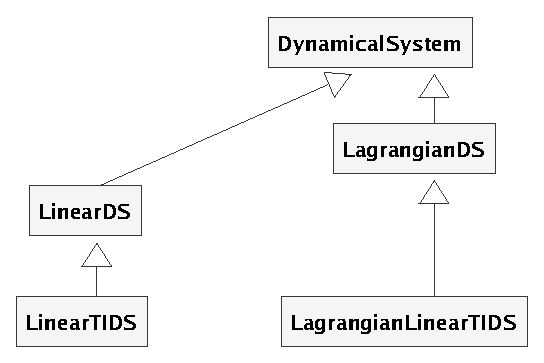
\includegraphics[width=0.3\textwidth]{./DSClassDiagram.eps}
  \label{DSDiagram}
\end{figure}
% DYNAMICAL SYSTEMS

\section{Construction}

Each constructor must:
\begin{itemize}
\item initialize all the members of the class and of the top-class if it exists
\item allocate memory and set value for all required inputs
\item allocate memory and set value for optional input if they are given as argument (in xml for example)
\item check that given data are coherent and that the system is complete (for example, in the LagrangianDS
if the internal forces are given as a plug-in, their Jacobian are also required. If they are not given, this leads to an exception).
\end{itemize}

No memory allocation is made for unused members $\Rightarrow$ requires if statements in simulation.  (if!=NULL ...).\\

\subsection{DynamicalSystem}

\bf{Required data:}\\
n, x0, f, jacobianXF \\
\bf{Optional:}\\
T,u \\

\bf{Always allocated in constructor:} \\
x, x0, xFree, r, rhs, jacobianXF

Warning: default constructor is always private or protected and apart from the others and previous rules or remarks do not always apply to it. 
This for DS class and any of the derived ones. 

\subsection{LagrangianDS}

\bf{Required data:}\\
ndof, q0, velocity0, mass \\
\bf{Optional:}\\
fInt and its Jacobian, fExt, NNL and its Jacobian. \\

\bf{Always allocated in constructor:} \\
mass, q, q0, qFree, velocity, velocity0, velocityFree, p. \\
All other pointers to vectors/matrices are set to NULL by default. \\
Memory vectors are required but allocated during call to initMemory function. 

Various rules:
\begin{itemize}
\item fInt (NNL) given as a plug-in $\Rightarrow$ check that JacobianQ/Velocity are present (matrices or plug-in)
\item any of the four Jacobian present $\Rightarrow$ allocate memory for block-matrix jacobianX  (connectToDS function)
\item 
\end{itemize}

check: end of constructor or in initialize? \\
computeF and JacobianF + corresponding set functions: virtual or not? \\


\section{Specific flags or members}

\begin{itemize}
\item isAllocatedIn: to check inside-class memory allocation
\item isPlugin: to check if operators are computed with plug-in or just directly set as a matrix or vector
\item workMatrix: used to save some specific matrices in order to avoid recomputation if possible (inverse of mass ...)
\end{itemize}

\section{plug-in management}
DynamicalSystem class has a member named parameterList which is a $map<string, SimpleVector*>$, ie a list of
pointers to SimpleVector*, with a string as a key to identified them. 
For example, $parametersList["mass"]$ is a SimpleVector*, which corresponds to the last argument given in 
mass plug-in function. \\
By default, each parameters vectors must be initialized with a SimpleVector of size 1, as soon as the plug-in is
declared. Moreover, to each vector corresponds a flag in isAllocatedIn map, to check if the corresponding vector has been 
allocated inside the class or not. \\ 
For example, in DynamicalSystem, if $isPlugin["vectorField"]==true$, then, during call to constructor or set function,
it is necessary to defined the corresponding parameter: \\
$parametersList["vectorField"] = new SimpleVector(1)$ \\
and to complete the $isAllocatedIn$ flag: \\
$isAllocatedIn["parameter_for_vectorField"] = true$. \\

\end{document}
